\documentclass[../../../../main.tex]{subfiles}
\begin{document}

\begin{flushright}
\footnotesize\textit{【自動文字起こし・要確認】}
\end{flushright}

[解] 図形は$x$軸対称だから、
$OQ \perp O'Q$ でもある。
$P, Q$ が $x \le 0$ にある時明らか
かに $OP \perp O'P$ とはなら
ないから... $\star$、$P, Q$ が $x \ge 0$ に
ある時のみ考える。円 $C'$ の
半径 $r'$ とし、$P$ から$x$軸への
垂足 $M$, $\angle POM = \alpha$, $\angle PO'M = \beta$ とおく ($0 < \alpha, \beta < \frac{\pi}{2}$) と題意から

$\begin{cases}
r^2 + r'^2 = 1 & \cdots \text{①} \\
r \sin \alpha = r' \sin \beta & \cdots \text{②} \\
\alpha + \beta = \pi/2 & \cdots \text{③}
\end{cases}$

このもとで、
($\square OP O' Q$ の面積 $S_1$) $= r r'$ \\
($D \cap D'$ の面積 $S_2$) $= \frac{1}{2} \cdot 2\alpha r^2 + \frac{1}{2} \cdot 2\beta r'^2 - r r'$
$= \alpha r^2 + \beta r'^2 - r r'$

だから題意の面積 $S(r)$ として
$S(r) = S_1 - S_2 = 2 r r' - (\alpha r^2 + \beta r'^2)$

②の両辺を、2乗して、
$r^2 \sin^2 \alpha = r'^2 \sin^2 \beta \quad \cdots \text{④}$

①④から
$r^2 = \frac{\sin^2 \beta}{\sin^2 \alpha + \sin^2 \beta}$, \quad $r'^2 = \frac{\sin^2 \alpha}{\sin^2 \alpha + \sin^2 \beta}$

$r r' > 0$ から
$r r' = \frac{\sin \alpha \sin \beta}{\sin^2 \alpha + \sin^2 \beta} \quad (\because \text{以上より } 0 < \alpha, \beta < \pi/2 \text{ を用いた})$

これらを $S(r)$ に代入して
$S(r) = \frac{1}{\sin^2 \alpha + \sin^2 \beta} \left[ 2 \sin \alpha \sin \beta - \alpha \sin^2 \beta - \beta \sin^2 \alpha \right]$

③を代入し、$S = \sin \alpha, C = \cos \alpha$ として
\begin{align*}
S(r) &= 2SC - \alpha C^2 - (\frac{\pi}{2} - \alpha) S^2 \\
&= 2SC + \alpha (S^2 - C^2) - \frac{\pi}{2} S^2 \equiv T(\alpha)
\end{align*}

\begin{align*}
T'(\alpha) &= 2 \cos 2\alpha - \cos 2\alpha + 2\alpha \sin 2\alpha - \frac{\pi}{4} \cdot 2 \sin 2\alpha \\
&= \cos 2\alpha + 2(\alpha - \frac{\pi}{4}) \sin 2\alpha
\end{align*}

\begin{align*}
T''(\alpha) &= -2 \sin 2\alpha + 2 \sin 2\alpha + 4(\alpha - \frac{\pi}{4}) \cos 2\alpha \\
&= 4(\alpha - \frac{\pi}{4}) \cos 2\alpha \le 0
\end{align*}

だから、$T'(\alpha)$ は単調減少。これと $T'(\pi/4) = 0$ から
下表をえる。

\begin{center}
\begin{tabular}{|c|c|c|c|c|c|}
\hline
$\alpha$ & $0$ & $\cdots$ & $\pi/4$ & $\cdots$ & $\pi/2$ \\
\hline
$T'$ & & $+$ & $0$ & $-$ & \\
\hline
$T$ & & $\nearrow$ & & $\searrow$ & \\
\hline
\end{tabular}
\end{center}

よって $T(\alpha)$ は、$\alpha = \pi/4$ で max $1 - \frac{\pi}{4}$ をとる。

\begin{center}
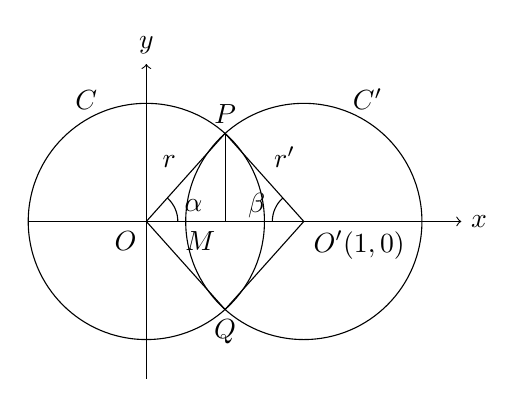
\begin{tikzpicture}
\draw[->] (-1.5,0) -- (4,0) node[right] {$x$};
\draw[->] (0,-2) -- (0,2) node[above] {$y$};
\draw (0,0) circle (1.5);
\draw (2,0) circle (1.5);
\coordinate (O) at (0,0);
\coordinate (O') at (2,0);
\coordinate (P) at (1, 1.118);
\coordinate (Q) at (1, -1.118);
\coordinate (M) at (1, 0);

\draw (O) -- (P) node[midway, above left] {$r$};
\draw (O') -- (P) node[midway, above right] {$r'$};
\draw (O) -- (Q);
\draw (O') -- (Q);
\draw (P) -- (M);
\node[above] at (P) {$P$};
\node[below] at (Q) {$Q$};
\node[below left] at (O) {$O$};
\node[below right] at (O') {$O'(1,0)$}; 
\node[below left] at (M) {$M$};
\node[above left] at (-0.5, 1.3) {$C$};
\node[above right] at (2.5, 1.3) {$C'$};
\draw (0.4,0) arc (0:48:0.4);
\node at (0.6, 0.2) {$\alpha$};
\draw (1.6,0) arc (180:132:0.4);
\node at (1.4, 0.2) {$\beta$};
\end{tikzpicture}
\end{center}

\vspace{1em}
\noindent
\framebox{
\begin{minipage}{0.9\textwidth}
$\star$ ベクトル表示で内積とればすぐわかる \\
全部文字おいてやったけど、天下り的に座標設定して...でもいいかも。\\
けっきょく、①から$r$を消して、多分同じになる
\end{minipage}
}

\vspace{1em}
\begin{center}
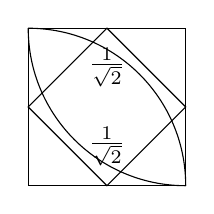
\begin{tikzpicture}
\draw (-1, -1) rectangle (1, 1);
\draw (-1,0) -- (0,1) -- (1,0) -- (0,-1) -- cycle;
\draw (-1,1) arc (180:270:2);
\draw (1,-1) arc (0:90:2);
\node at (0, 0.5) {$\frac{1}{\sqrt{2}}$};
\node at (0, -0.5) {$\frac{1}{\sqrt{2}}$};
\end{tikzpicture}
\end{center}
\begin{align*}
\square &= \frac{1}{2} \cdot 2 \cdot \frac{\pi}{4} \cdot \left(\frac{1}{\sqrt{2}}\right)^2 - \left(\frac{1}{\sqrt{2}}\right)^2 = \frac{\pi}{4} - \frac{1}{2} \\
\square &= \frac{1}{2} \\
&\Rightarrow OK!!
\end{align*}

\end{document}
